\chapter{Methodology}
\label{chapter:methodology}
In this chapter, we present our proposed methodology, including the methods and techniques used to address our research questions. Our methodology consists of four main components: (1) data exploration, preprocessing, and augmentation to prepare the OpenML dataset descriptions, (2) a novel tag generation pipeline that extends BERTopic with large language models and zeroshot classification, (3) automated evaluation and optimization using topic coherence, diversity metrics, and baseline comparisons, and (4) human evaluation through a user study complemented by large-scale automated evaluation. We provide a detailed description of each component, along with their limitations and how they address our research questions.

\section{Data exploration, preprocessing and augmentation}
\label{sec:data_exploration}
\subsection{Exploratory data analysis}
First, an exploratory data analysis (EDA) will be conducted to understand the characteristics of the OpenML dataset descriptions. \cref{fig:dataset_examples} shows an example of an OpenML dataset, which includes a dataset name (\texttt{COVID-19-Rio-de-Janeiro-(City)}), a dataset description (\texttt{Context - World Health Organization (WHO)...}), tags (\texttt{Computer Systems, Machine Learning}), and columns (\texttt{Date, Hour, Neighborhood, Cases, Deaths, Recovered}).

This analysis will be unstructured, discovering patterns in the data in an exploratory manner, using statistical and visual methods. The goal of the EDA is to gain insights into the dataset descriptions, such as their length, vocabulary, distribution of words, etc. This information will help us understand the nature of the data and identify any preprocessing steps that may be necessary to improve the quality of the descriptions.

\begin{figure}[h]
    \centering
    \subfloat[Dataset information]{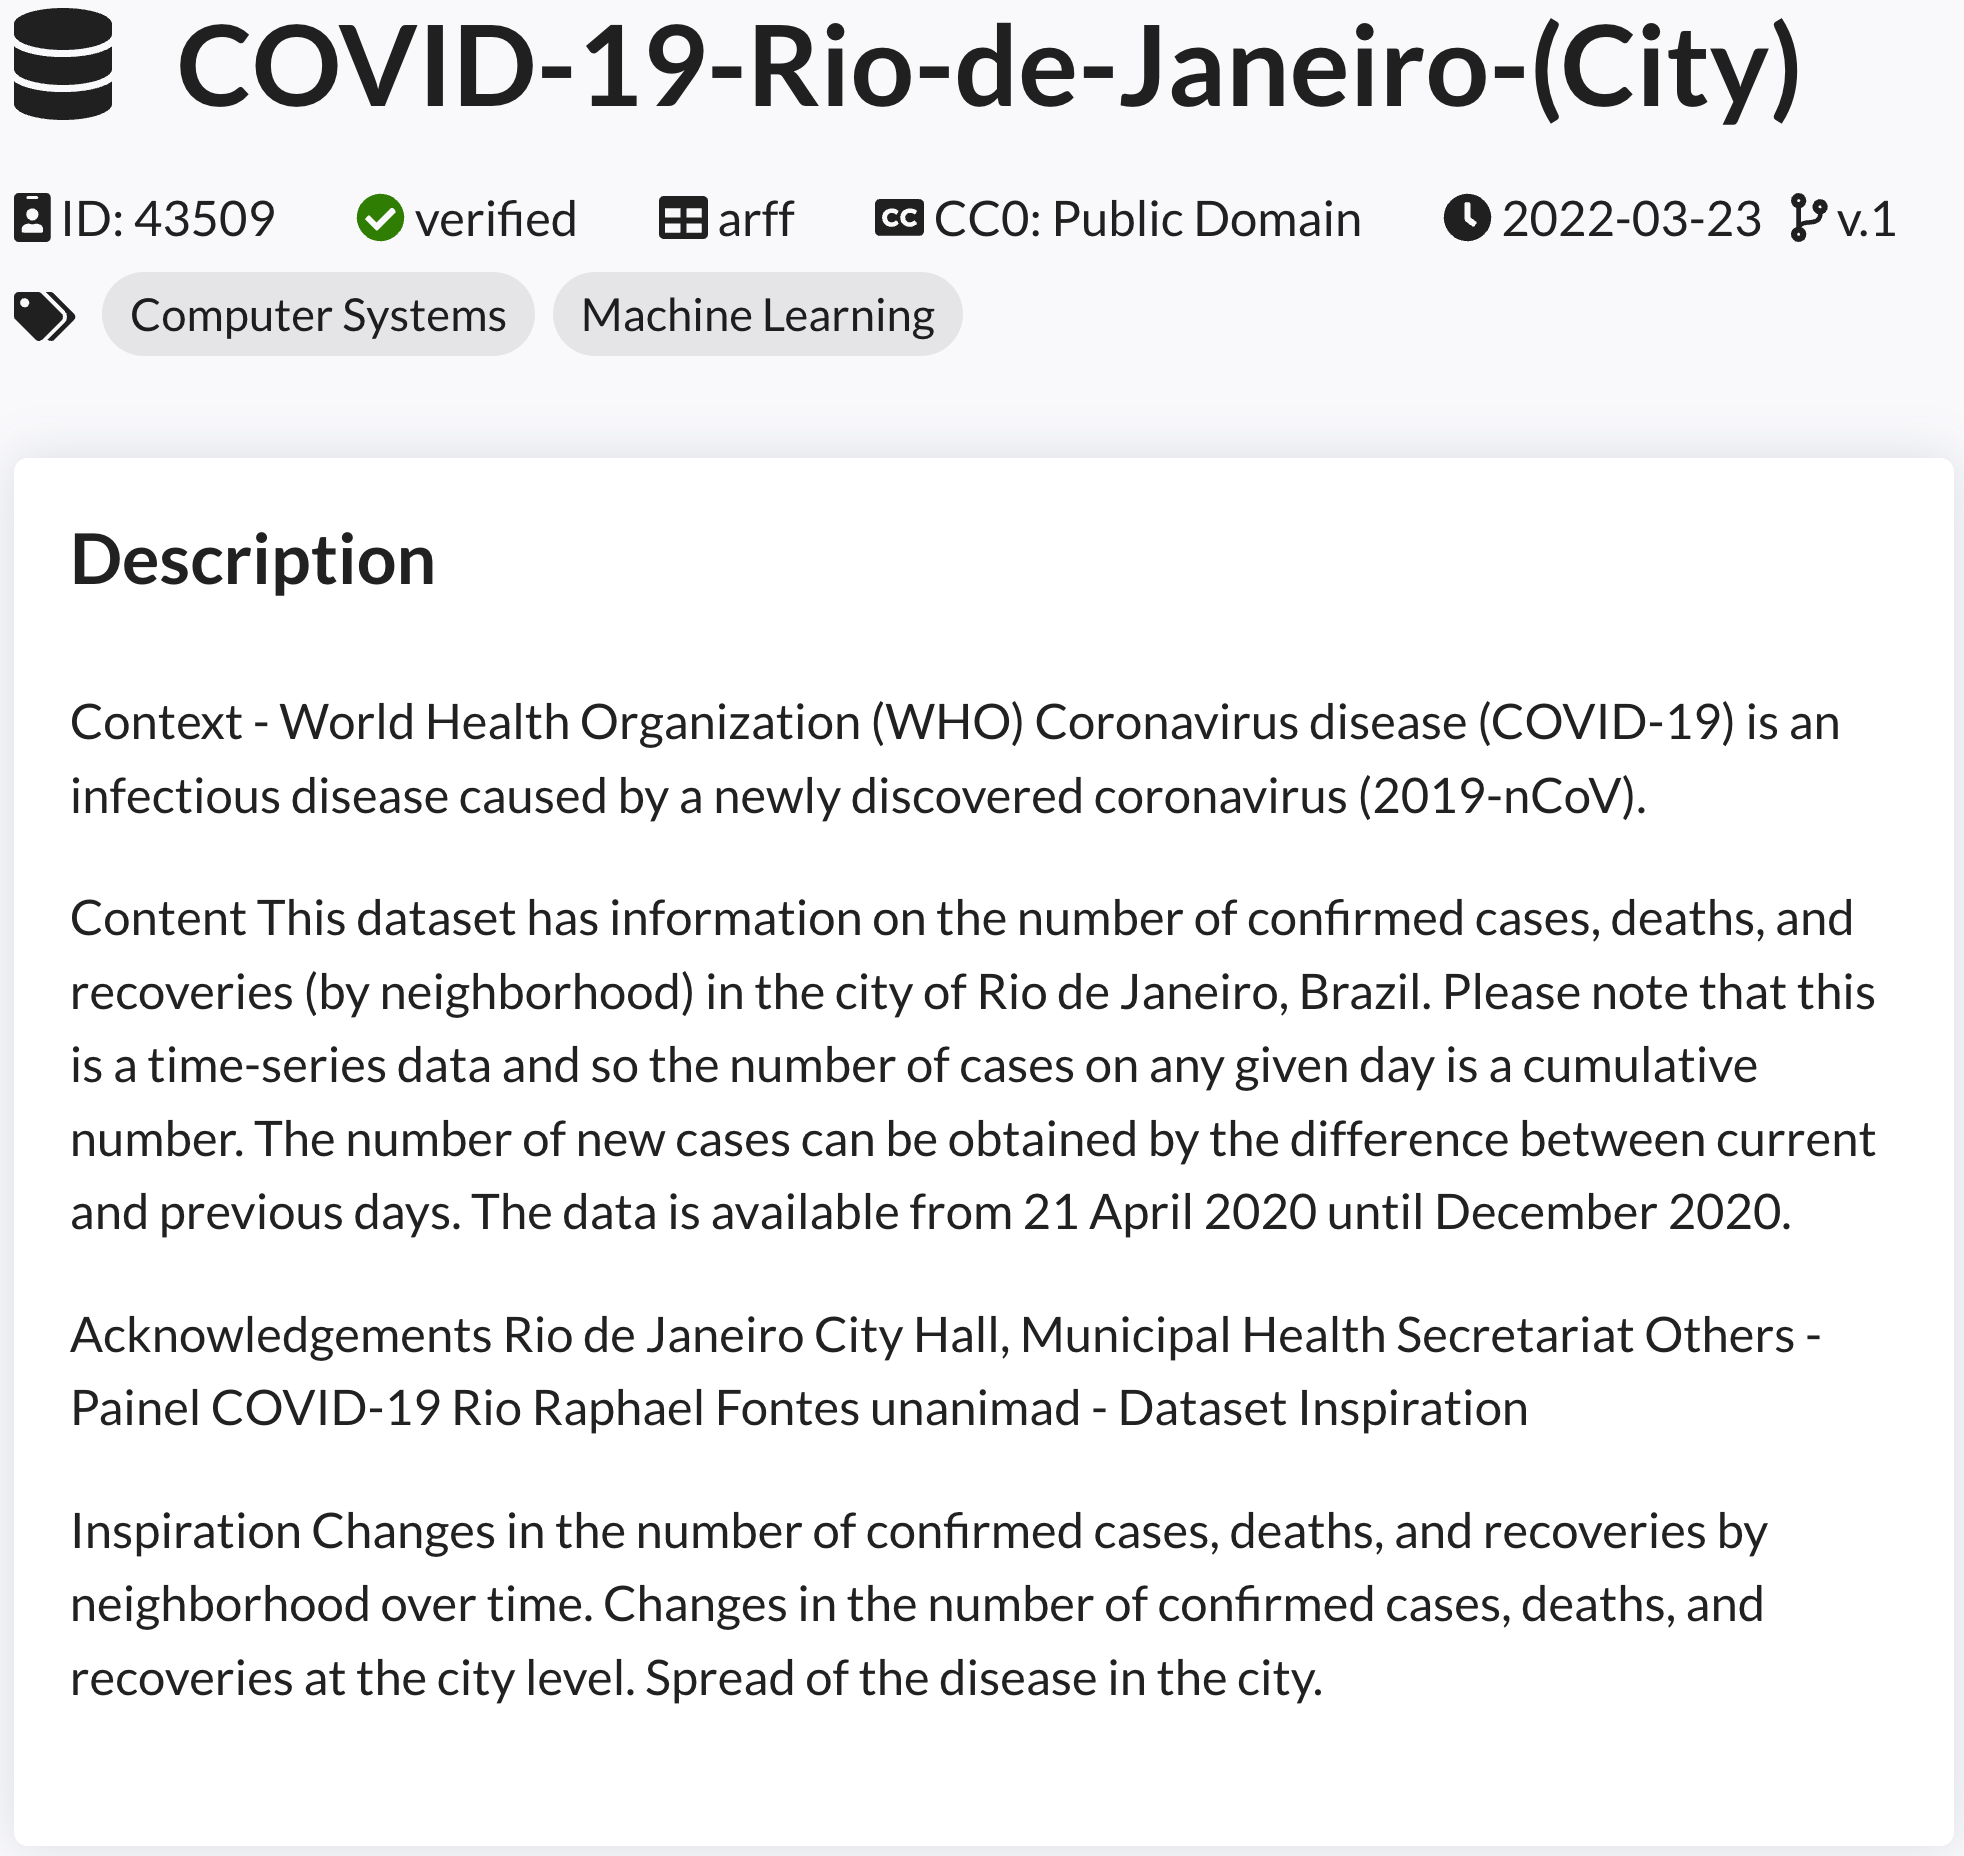
\includegraphics[width=0.49\textwidth]{figures/dataset_example.png}\label{fig:dataset_example}}
    \hfill
    \subfloat[Dataset columns]{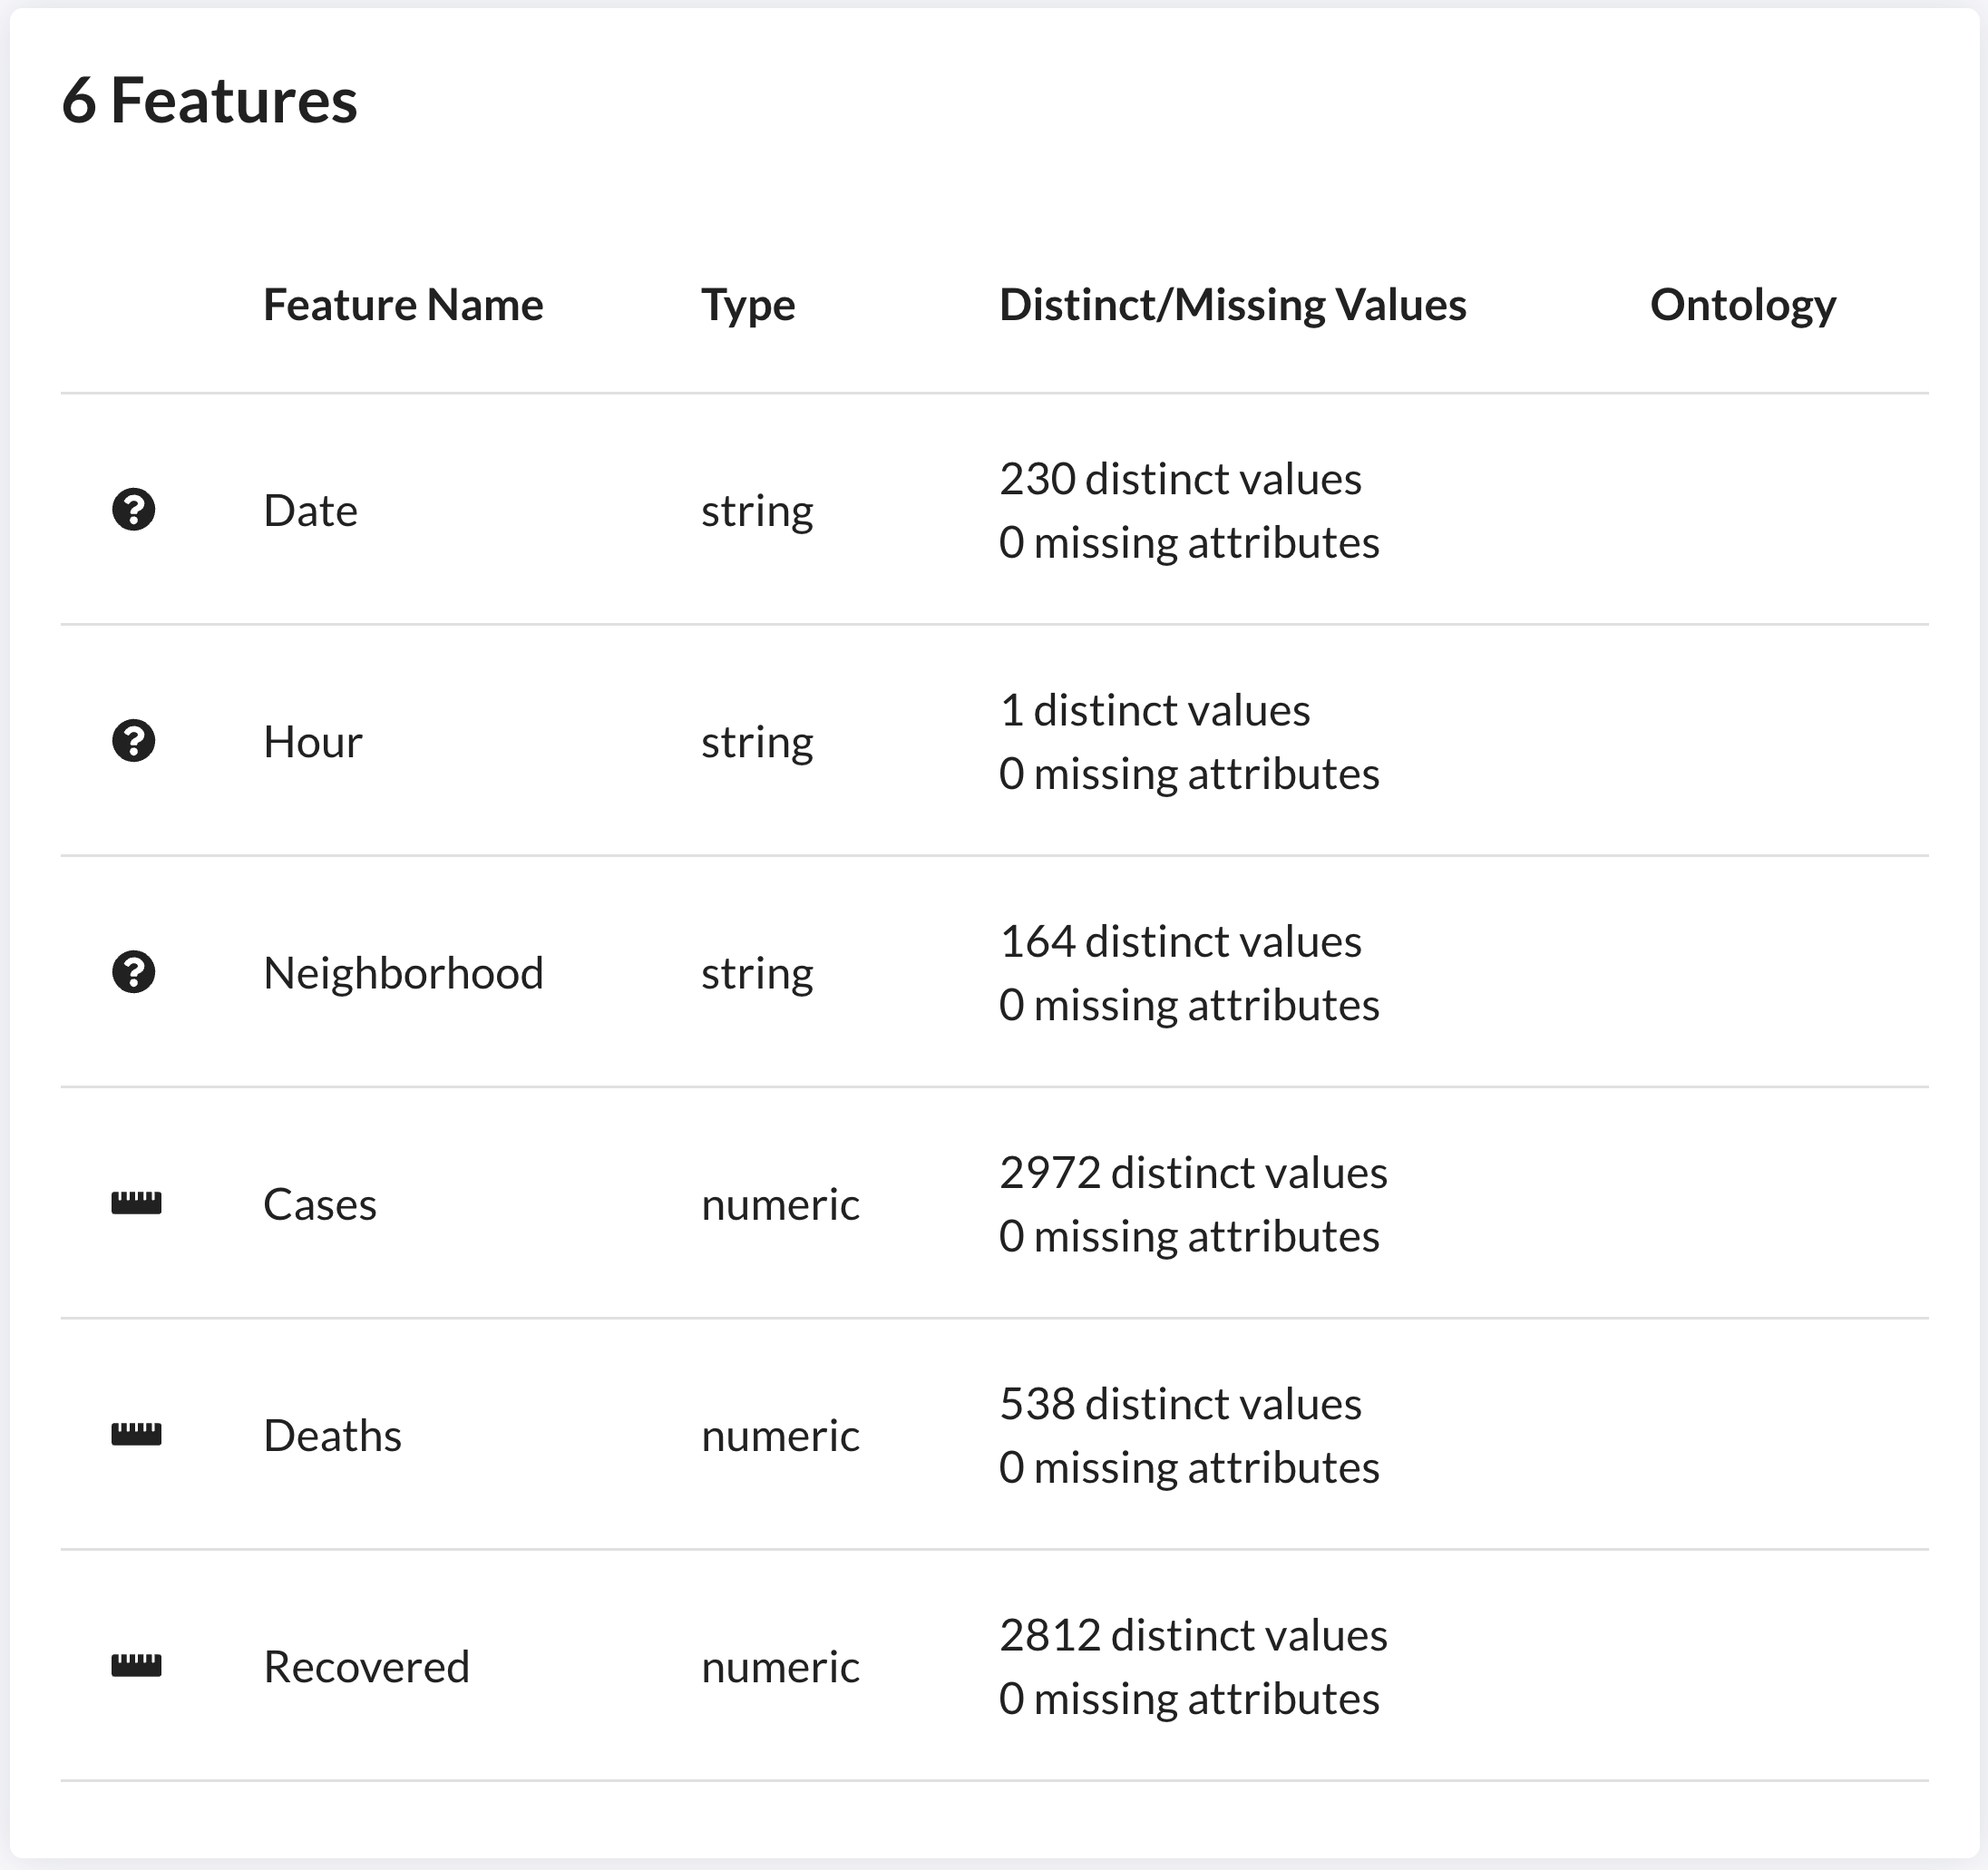
\includegraphics[width=0.49\textwidth]{figures/dataset_example_features.png}\label{fig:dataset_example_features}}
    \caption{OpenML dataset example}
    \label{fig:dataset_examples}
\end{figure}

\subsection{Data preprocessing}
After the EDA, the dataset descriptions will undergo preprocessing to prepare them for the topic modeling process. For traditional topic models like LDA and NMF, which rely on sparse representations of text (e.g., bag-of-words or TF-IDF) and do not inherently understand semantic relationships between words, several preprocessing steps are necessary:

\begin{itemize}
    \item Stemming and lemmatization: These reduce words to their root or base form (e.g., \textit{running} to \textit{run}), ensuring that different forms of the same word are treated as identical. This is important for models that treat words as discrete tokens, as it helps capture true word frequencies.
    \item Stop-word removal: Common words like \textit{the}, \textit{and}, \textit{is} are removed as they carry little semantic meaning and can dominate frequency-based representations.
    \item Tokenization: Text is split into individual tokens (words or subwords), creating the discrete units that these models operate on.
\end{itemize}

Modern embedding-based models like Top2Vec and BERTopic typically do not require these preprocessing steps, as they use embedding models that can capture semantic meaning and handle word variations naturally.

\subsection{Data augmentation}
In addition to the original dataset descriptions, we will explore the possibility of augmenting the data with additional information. This could include metadata such as dataset name, tags, features (column names), scraping from the original dataset if available. This additional information can provide context and background to the descriptions, which may help improve the quality of the topics extracted by the topic model.

\section{Tag generation}
\label{sec:tag_generation}

\subsection{Pipeline}
\label{sec:tag_generation_pipeline}
In this subsection, we introduce our model, which is, in fact, a pipeline comprising multiple submodels and techniques. We shall henceforth refer to this pipeline as our \textit{proposed model}.

Steps 1-3 involve data preprocessing to prepare the data for the proposed model. We shall refer to steps 5-8 as the \textit{Base BERTopic model}. It includes dimensionality reduction, clustering, bag-of-words and c-TF-IDF. Finally, steps 9 and 10 represent our improvements to the base model, introducing an approach that, to the best of our knowledge, is novel within the literature. Additionally, we provide an explanation of which steps are computationally efficient and which are more expensive.

\begin{figure}[h]
    \centering
    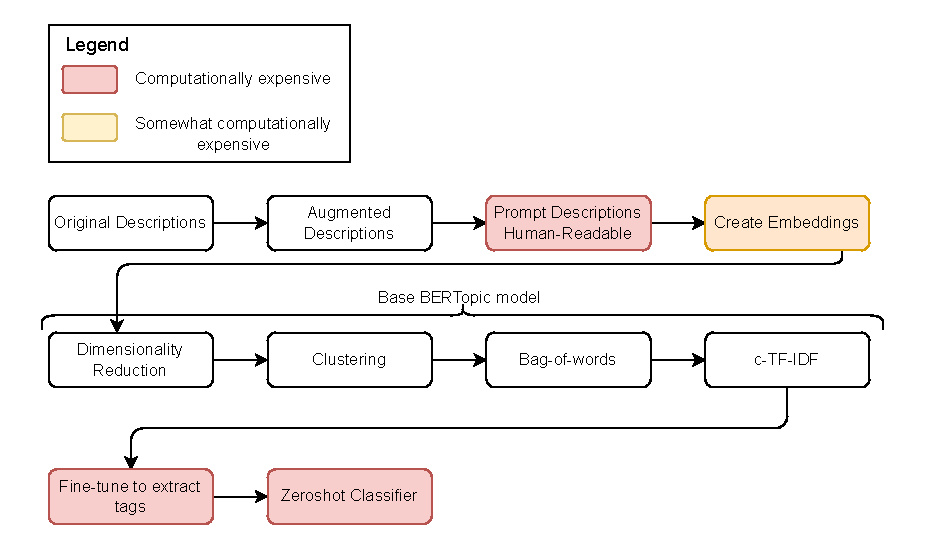
\includegraphics[width=\textwidth]{figures/tag_generation_pipeline.pdf}
    \caption{Tag generation pipeline (\textit{proposed model})}
    \label{fig:tag_generation_pipeline}
\end{figure}

To explain the pipeline illustrated in \cref{fig:tag_generation_pipeline} in more detail, we provide a step-by-step description of the process:

\begin{enumerate}
    \item \textbf{Original Descriptions}: The input to the pipeline is a set of original dataset descriptions. These come from the OpenML dataset and are used as the basis for generating tags.
    \item \textbf{Augmented Descriptions}: The OpenML dataset descriptions come with metadata such as dataset name, tags, features (column names) and some of them link to the original dataset, which can be used to scrape (extract) additional information. These are used to augment the dataset descriptions.
    \item \textbf{Prompt Descriptions Human-Readable}: Augmented descriptions are rewritten to be more human-readable via an LLM and prompt engineering. This is because the original descriptions are often in a technical format that is not easily interpretable by humans. Since LLMs are trained on large text corpora, they work best with human-readable (natural language) text.
    
    Additionally, we design the prompt to extract \textit{keyword tags} from each individual description. These tags are directly mentioned within the description and are typically highly specific to it. For instance, if a description includes the terms "US elections," "voting," and "candidates," these would be considered keyword tags.

    \cref{fig:augmented_description_before,fig:augmented_description_after} show an example of an augmented description before and after the augmentation and rewriting process.

    \item \textbf{Create Embeddings}: Embeddings for each description are created using a pre-trained embedding model.
    \item \textbf{Dimensionality Reduction}: The dimensionality of the embeddings is reduced to cure the curse of dimensionality.
    \item \textbf{Clustering}: The reduced embeddings are clustered to group similar descriptions together. The output of this step is clusters, which represent our topics. Each cluster contains a set of descriptions (which we now call \textit{representative documents}) that are similar to each other.
    \item \textbf{Bag-of-words}: The descriptions in each cluster are converted to a bag-of-words representation, ignoring common words such as "the", "and", etc.
    \item \textbf{c-TF-IDF}: The bag-of-words representation is used to calculate the c-TF-IDF score for each word in each cluster. This score is used to rank the words in each cluster.
    \item \textbf{Fine-tune To Extract Tags}: For each topic, we have representative documents (from the clustering step) and representative words (from the c-TF-IDF step). We prompt engineer a question that asks an LLM to generate tags for each cluster. The generated tags are categorized as \textit{regular tags} and \textit{overarching tags}.

    \textit{Regular tags} refer to tags that frequently appear among the representative documents and words. \textit{Overarching tags} capture the broader, more general theme of the cluster. For example, if a cluster pertains to \textit{US elections} and the representative documents contain the word \textit{election} while the representative words include \textit{candidate}, a possible regular tag could be \textit{election candidate}, whereas the overarching tag might be \textit{politics}.

    As context, we feed the LLM with the top \textit{k} representative documents and the top \textit{m} representative words for each topic. This results in tags that are common among the representative documents and representative words, and hence are representative of the topic.

    We prompt engineer a question that asks the LLM to generate tags for each cluster, and provide a few examples. This is known as few-shot prompting, which has been shown to improve the performance of LLMs on specific tasks compared to zero-shot or one-shot prompting \cite{touvron_llama_2023,brown_language_2020,min_rethinking_2022,sivarajkumar_empirical_2024}.
    \item \textbf{Zeroshot Text Classifier}: Each description can in reality be contained in multiple clusters (topics) if we use a soft clustering approach such as HDBSCAN. In this step, we get the top \textit{n} most likely clusters for each description. Then, for each description, we get the tags for each of the top \textit{n} clusters in a set. 
    
    The advantage provided by this step is that a description can be contained in multiple clusters, and we can get tags for each of these clusters. This is important because a description may contain multiple topics, and we want to ensure that we capture all of them. For instance, we may have a cluster about \textit{politics} and a cluster about \textit{sports}. A description about the Olympics may be contained in both of these clusters, and we want to ensure that we get tags for both of these clusters.
    
    We then feed this set of tags to a zeroshot text classification model, which returns confidences from 0 to 1 for whether each tag describes the description. This step is crucial for filtering out irrelevant tags for each description. For instance, if a description about diabetes and a description about cancer are both contained in the same topic (which may be, for example, \textit{medical conditions}), we want to ensure that the tags for the cancer description are not assigned to the diabetes description. Furthermore, the description about diabetes may be contained in another topic that cancer is not in, such as \textit{nutrition}. In this case, we want to ensure that the tags in \textit{nutrition} are not assigned to the cancer description, but are assigned to the diabetes description.

\end{enumerate}

\begin{figure}[h]
    \centering
    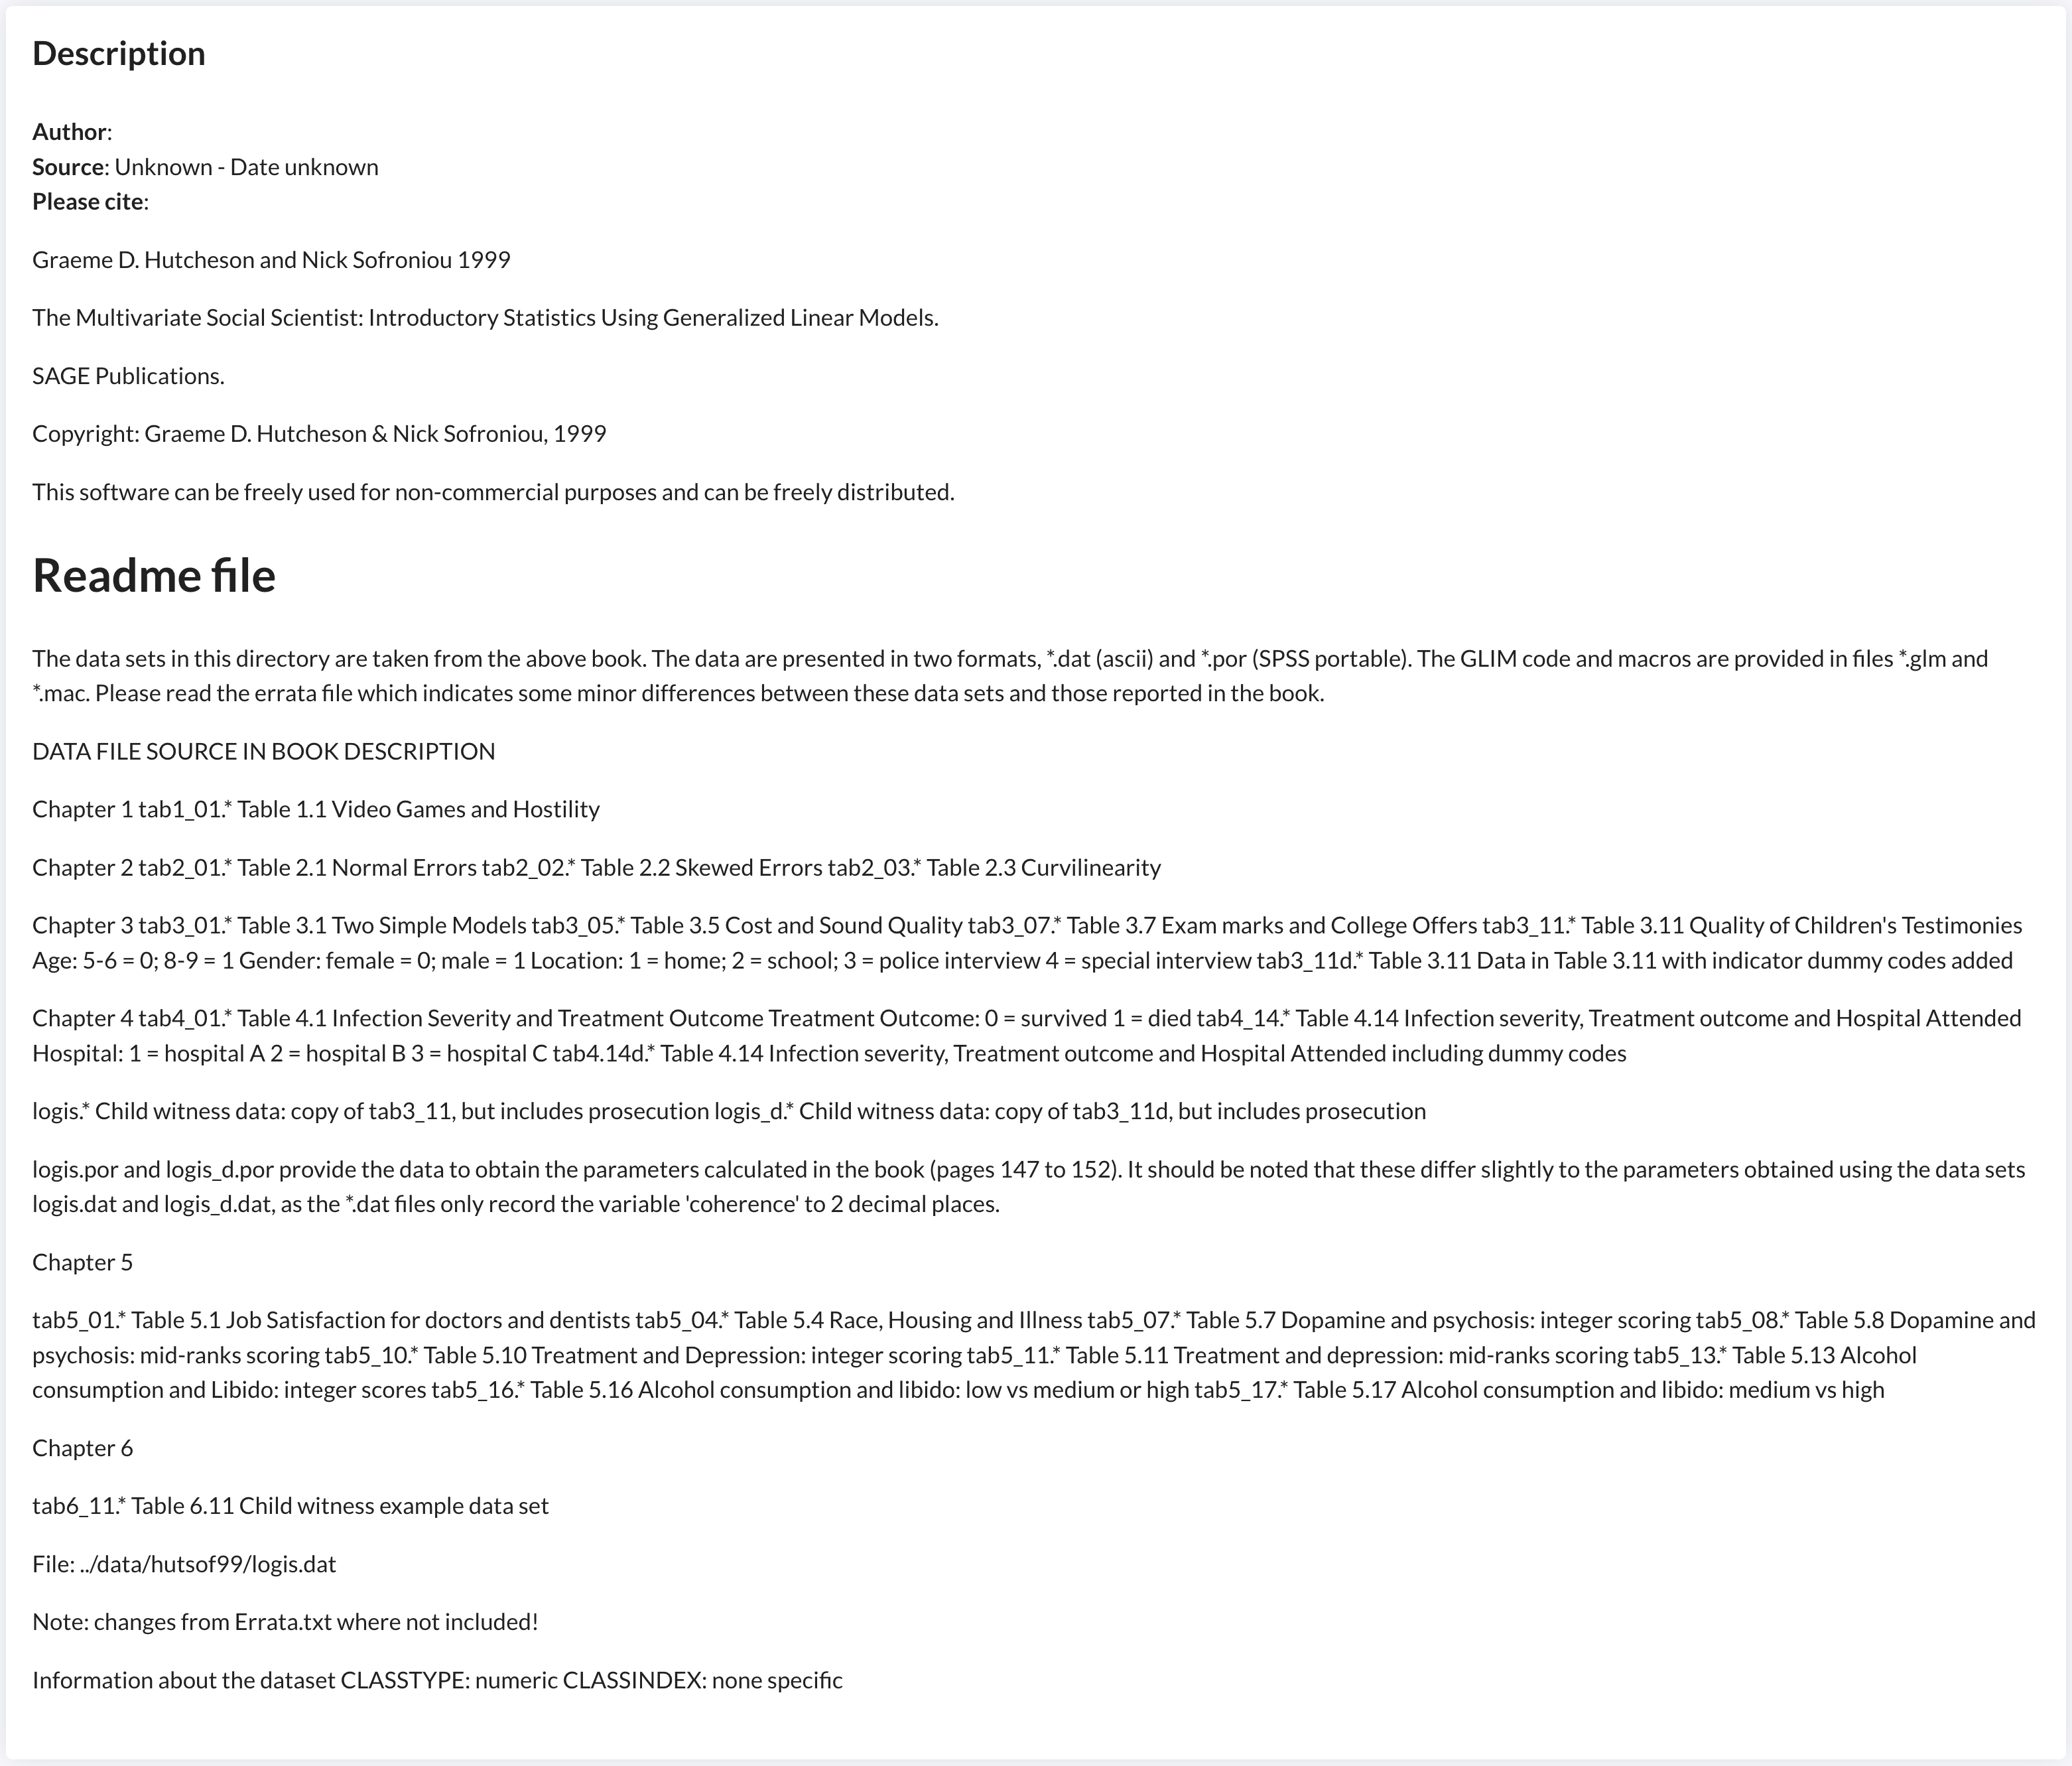
\includegraphics[width=\textwidth]{figures/augmented_description_before.png}
    \caption{Augmented dataset description example (before)}
    \label{fig:augmented_description_before}
\end{figure}

\begin{figure}[h]
    \centering
    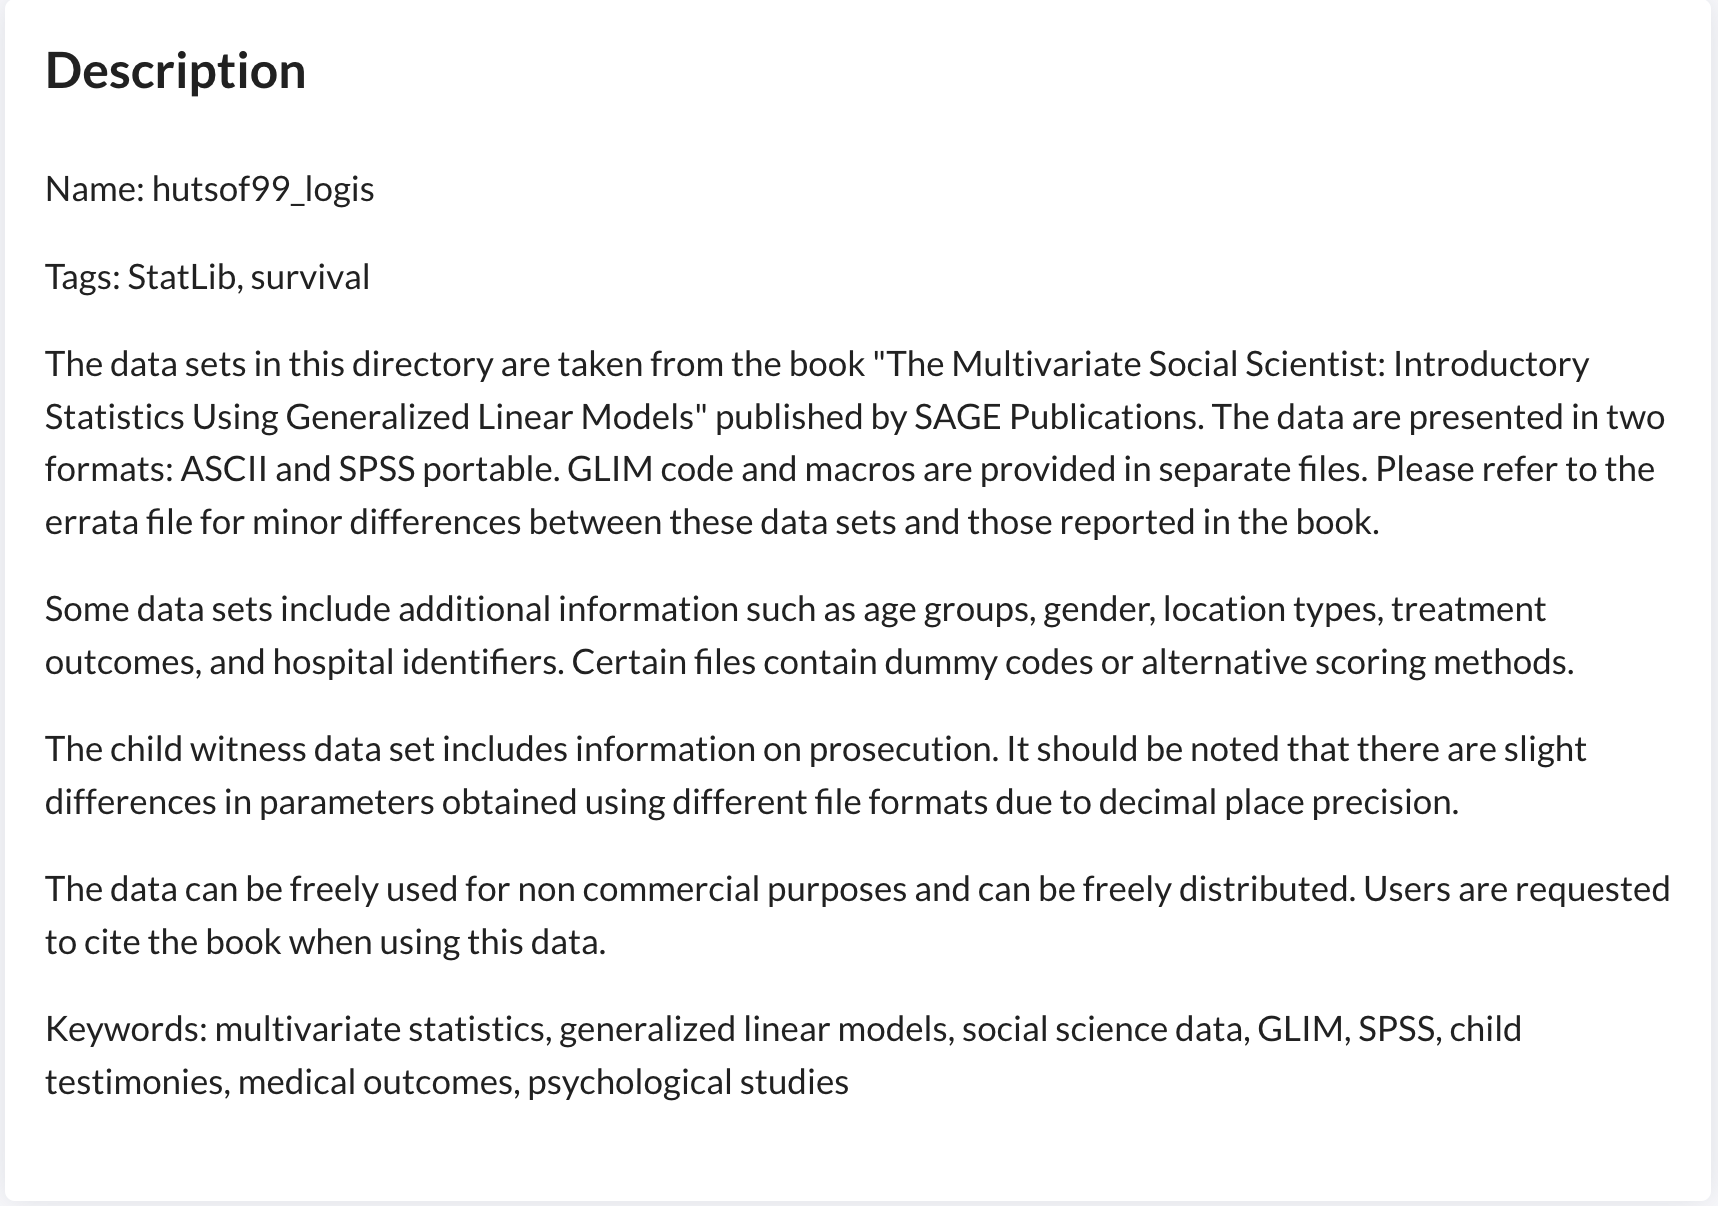
\includegraphics[width=0.65\textwidth]{figures/augmented_description_after.png}
    \caption{Augmented dataset description example (after)}
    \label{fig:augmented_description_after}
\end{figure}

\subsection{Rationale}
\label{sec:rationale}
In this subsection, we aim to provide a rationale for the proposed model.

\subsubsection{Proposed model}
We provided our rationale for steps 1 and 2 in \cref{sec:data_exploration}, and for step 3 in \cref{sec:tag_generation_pipeline}. Steps 4-8 are part of the Base BERTopic model, a well-established topic modeling technique proven effective across various datasets. Hence, we will focus on steps 9 and 10, which are novel contributions to the existing literature.

Without steps 9 and 10, we would need to solely rely on the c-TF-IDF representation from step 8 to extract tags. For background on c-TF-IDF, the reader may refer to \cref{sec:bag_of_words,sec:topic_representation}. This c-TF-IDF representation has several limitations:
\begin{itemize}
    \item It is based on the bag-of-words representation of the descriptions, which may not capture the full semantic meaning of the text. The c-TF-IDF calculation relies on word frequencies in the descriptions, which is a naive way of capturing word importance in the context of topics, as it does not consider the relationships between words.
    \item It depends on the top words in each cluster, which may not always be representative of the topics. For instance, if a cluster's top words are \textit{election} and \textit{candidate}, these words may not capture the broader theme of \textit{politics}.
\end{itemize}

The LLM helps address these limitations by generating tags that better represent the topics. Trained on a large corpus of text, it can capture semantic relationships between words. By providing the LLM with the top representative documents and words for each cluster, we can prompt it to generate more representative topic tags. The LLM can identify broader themes and generate more descriptive tags, improving tag quality for users.

If we only use step 9 and not step 10, we have two significant limitations:
\begin{itemize}
    \item We miss the opportunity to capture the multiple topics a description may belong to.
    \item We cannot filter out irrelevant tags for each description, as not all cluster tags may be relevant to every description within that cluster, as illustrated by the example in step 10 of \cref{sec:tag_generation_pipeline}.
\end{itemize}

Conversely, if we only use step 10 and not step 9, we must rely on the c-TF-IDF representation to classify tags. As discussed, this representation has several limitations, and using it alone may result in lower quality and less representative tags. By combining steps 9 and 10, we leverage the strengths of both LLMs and zeroshot classifiers to generate tags that are higher quality, more representative, and more relevant to the descriptions.

\subsubsection{Advantages over naive LLM approaches}
A naive approach would be to simply feed each individual description to an LLM and ask it to extract tags. However, our proposed pipeline offers several advantages over this approach:

\begin{enumerate}
    \item \textbf{Contextual Consistency}: By clustering similar descriptions together, our model develops a broader understanding of related topics. This allows it to generate more consistent and contextually relevant tags across similar descriptions. For example, if we have two similar descriptions about image classification using convolutional neural networks, a naive approach might tag one with \textit{CNN} and another with \textit{computer vision}, while our approach would recognize their similarity and consistently apply both relevant tags to both descriptions. A naive approach, analyzing descriptions in isolation, would generate inconsistent tags for similar descriptions due to lacking this broader context and varying interpretations of individual texts.
    
    \item \textbf{Multi-level Tag Generation}: Our approach generates tags at multiple levels of specificity:
    \begin{itemize}
        \item Keyword tags from individual descriptions (step 3)
        \item Regular tags that are common across cluster members (step 9)
        \item Overarching tags that capture broader themes (step 9)
    \end{itemize}
    A naive LLM approach, working with single descriptions, would focus on explicitly mentioned concepts in individual descriptions and miss broader thematic connections.
    
    \item \textbf{Cross-validation}: The combination of clustering and zeroshot classification provides a form of cross-validation for tag relevance. Tags are not just extracted from individual descriptions but are validated against similar descriptions within the same cluster and verified through the zeroshot classifier. For example, consider a cluster about weather forecasting where one of the descriptions briefly mentions \textit{neural networks}. While the LLM might generate \textit{neural networks} as a tag for the cluster, the zeroshot classifier would likely assign it a low confidence score for other descriptions in the cluster, since it is not their main focus. This helps filter out irrelevant tags, thus improving tag quality. 
    
    \item \textbf{Computational Efficiency}: While our pipeline uses LLMs, it does so more efficiently by processing clusters rather than individual descriptions. In a naive approach, we would need $n$ LLM calls for $n$ descriptions, while our clustering approach requires only $k$ calls, where $k$ is the number of clusters ($k < n/2$, $k < n/3$, or even $k < n / 5$, depending on the clustering parameters). This significantly reduces the number of LLM calls needed, particularly for large datasets with many similar descriptions. For large clusters, we can further optimize token usage by selecting only the most representative documents (e.g., using 50 instead of all 80 descriptions in a cluster) while still maintaining the cluster's semantic meaning through the remaining representative descriptions. Similarly, we can truncate individual description lengths while preserving the overall topic through the collective context of the cluster. In contrast, with a naive LLM approach, truncating or dropping parts of individual descriptions would result in lost context and lower quality tags, as each description is processed in isolation without the benefit of related documents providing additional context.

\end{enumerate}

\subsubsection{Alternative configurations}
\label{sec:alternative_configurations}
The pipeline described in \cref{fig:tag_generation_pipeline} is one possible configuration for extracting tags from the OpenML dataset descriptions, which we believe will yield high-quality tags based on our reasoning. However, this pipeline is more computationally expensive due to the use of large language models and zeroshot text classifiers. To address this issue, we can consider alternative configurations that are more computationally efficient but may sacrifice some quality in tag generation.

\begin{enumerate}
    \item \textbf{Simpler Models}: We could use a smaller LLM for step 9 or a more lightweight zeroshot text classifier \cite{noauthor_moritzlaurerdeberta-v3-large-zeroshot-v20_2024} for step 10 to reduce computational cost. 
    
    Alternatively, the zeroshot classifier could be entirely replaced with a cheaper LLM. However, the confidence scores that the LLM outputs may not be as accurate as those from the zeroshot classifier, since the latter is specifically designed for text classification tasks. This could result in lower tag quality by assigning irrelevant tags to descriptions or missing relevant tags.
    
    \item \textbf{Pipeline Modification}: Depending on computational constraints, we could modify the pipeline to use only the most essential steps. For instance:
    \begin{itemize}
        \item Removing the zeroshot classifier and relying solely on the LLM
        \item Using the zeroshot classifier without the LLM
    \end{itemize}
    However, we expect that eliminating either component would significantly reduce tag quality based on our reasoning in the previous sections, so we do not recommend this approach.
    
    \item \textbf{Skip Description Rewriting}: We could omit step 3, which involves rewriting augmented descriptions to be more human-readable. While this step enhances embedding quality and, consequently, tag quality, it is computationally expensive. If computational constraints become an issue, removing this step offers a reasonable trade-off.
    
    \item \textbf{Combined Generation and Filtering}: Instead of using a separate zeroshot classifier, we could modify the fine-tuning step (step 9) to simultaneously generate and filter tags. This approach would generate tags for a cluster and assign them to each description in one step. However, this would skip getting the top \textit{n} most likely clusters for each description, which could result in missing relevant tags for descriptions that belong to multiple clusters, thus reducing tag quality.
\end{enumerate}

We recommend maintaining the complete pipeline for initial evaluation to ensure high-quality tags, and only exploring these alternative configurations if computational constraints become problematic.

\section{Automated evaluation metrics and baselines}
\label{sec:automated_evaluation_methodology}
In order to evaluate the quality of the extracted topics, we will use a combination of automated evaluation metrics and comparison with baselines. These metrics and baselines will help us assess the performance of our model and compare it to existing topic modeling techniques. The following sections provide an overview of the metrics and baselines we will use in our evaluation.

\subsection{Metrics}
From the range of possible evaluation metrics for topic models — including quality, interpretability, stability, diversity, efficiency, and flexibility — we focus on three metrics that are most relevant to our use case and are supported by literature, as explained in \cref{sec:evaluation_metrics}. Most of the remaining metrics appear infrequently in the literature and will not be included in our evaluation. Among our selected metrics, all except the silhouette score are widely adopted in topic modeling research. However, as discussed in \cref{sec:evaluation_metrics}, these commonly used metrics have significant limitations \cite{doogan_topic_2021, hoyle_is_2021}, especially when it comes to newer topic modeling approaches such as neural models. Therefore, their results should be interpreted with caution.

\subsubsection{Topic coherence}
As explained in \cref{sec:topic_coherence}, topic coherence is a widely used metric for evaluating the quality of topics generated by topic models. It measures the semantic similarity between words in a topic and is based on the assumption that coherent topics contain words that are related to each other. As explained in \cref{sec:evaluation_metrics}, topic coherence has been shown to correlate with human judgment, so we will use it to assess the cohesion of the topics extracted by our model.

\subsubsection{Topic diversity}
Topic diversity (\cref{sec:topic_diversity}) is another important metric for evaluating topic models. It measures the extent to which topics are distinct from each other and do not overlap in terms of the words they contain. A diverse set of topics ensures that the model captures a wide range of themes and concepts present in the data. We will use topic diversity to evaluate the diversity of topics generated by our model.

\subsubsection{Silhouette score}
The silhouette score (\cref{sec:silhouette_score}) is a metric used to evaluate the quality of clusters in unsupervised learning. It measures how similar an object is to its own cluster (cohesion) compared to other clusters (separation). A high silhouette score indicates that the clusters are well-separated and that the objects within each cluster are similar to each other. We will use the silhouette score to evaluate the quality of the clusters generated by our model.

\subsection{Baselines}
In addition to the proposed model, we will compare the performance of the Base BERTopic model against several \textit{baseline models}. These baselines represent established or commonly used topic modeling techniques and will serve as a point of reference for evaluating the proposed model. 

It is important to note that only the Base BERTopic model can and will be evaluated using the automated evaluation metrics, not the whole pipeline. There are two reasons for this limitation. First, the proposed model is a pipeline that includes several submodels and techniques, making it difficult to evaluate the pipeline as a whole using automated metrics due to resource constraints. Second, coherence and diversity metrics are not directly applicable to the proposed model, as it generates tags rather than topics. Therefore, automated evaluation metrics will be used only up to the Base BERTopic model (step 8 in \cref{fig:tag_generation_pipeline}).

Additionally, BERTopic, on its own, automatically determines the final number of clusters (topics) based on the data, which is a significant advantage over traditional topic modeling techniques that require the number of topics to be specified in advance. However, when comparing the Base BERTopic model to baselines, we will use the same number of topics for all models to ensure a fair comparison. We do this by taking the clusters generated by BERTopic, and reducing them to the same number of topics as the baselines by merging clusters based on their similarity until the desired number of topics is reached. It is important to note that this process may result in a loss of information, as the original clusters may contain more nuanced distinctions than the merged topics, thus potentially disadvantaging BERTopic in the comparison.

The baselines we will consider include Latent Dirichlet Allocation (LDA), Non-negative Matrix Factorization (NMF), and Top2Vec (described in \cref{sec:latent_dirichlet_allocation,sec:non-negative_matrix_factorization,sec:top2vec}), and Contextualized Topic Models (CTM) \cite{bianchi_pre-training_2021, bianchi_cross-lingual_2021} which are a less popular, but still effective topic modeling approach. These models are widely used in the field of topic modeling and will provide a benchmark for evaluating the performance of our model.

\subsection{Automated evaluation pipeline}

\Cref{fig:data_pipeline} shows a flowchart of the automated evaluation pipeline, which contains the following sequential steps:

\begin{enumerate}

    \item \textbf{Data Fetching}: This is the first stage where dataset descriptions are downloaded from OpenML.

    \item \textbf{Data Preparation}: After fetching the data, the next step involves preparation by preprocessing and augmenting it. Data preparation ensures that the input to the topic model is of high quality, which is important for the success of the subsequent modeling steps. \\ The next step involves removing inadequate data points such as duplicates. Stop words are removed for models that require it (e.g., LDA, NMF). Additionally, the process includes stemming and lemmatization to normalize words to their base forms.

    \item \textbf{Topic Model}: In this step, the Base BERTopic model is applied to the prepared data.

    \item \textbf{Benchmark Models}: Concurrently with the Base BERTopic model, benchmark models are run. These models represent established or baseline approaches \cite{grootendorst_bertopic_2022, blei_latent_2001, shahnaz_document_2006, kasiviswanathan_emerging_2011, yan_learning_2013, angelov_top2vec_2020, bianchi_pre-training_2021, bianchi_cross-lingual_2021} to topic modeling against which the performance of the proposed topic model is compared.

    \item \textbf{Topic Labels}: The output from both the Base BERTopic model and the benchmark models are sets of topics, represented by a cluster of words that are characteristic of a particular topic.

    \item \textbf{Evaluation}: Finally, the performances of the Base BERTopic model and benchmark models are evaluated. This includes comparing the topic coherence, diversity and silhouette score.

\end{enumerate}

\begin{figure}[h]
    \centering
    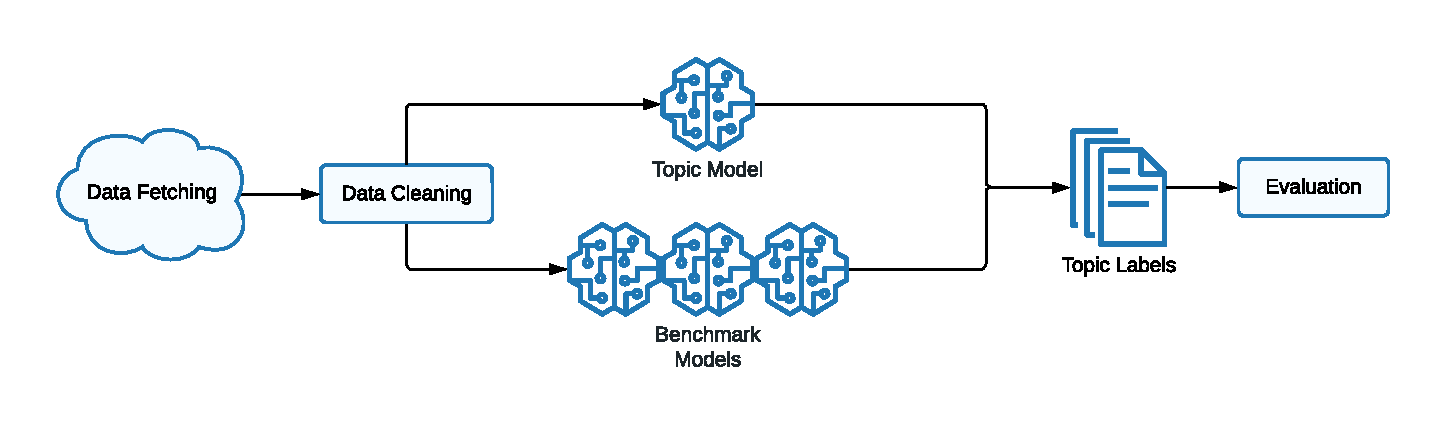
\includegraphics[width=\textwidth]{figures/data_pipeline.pdf}
    \caption{Data pipeline}
    \label{fig:data_pipeline}
\end{figure}

\subsection{Hyperparameter tuning}
\label{sec:hyperparameter_tuning}
As mentioned in \cref{sec:octis}, we will use Bayesian optimization to tune the hyperparameters of our Base BERTopic model. This process will involve selecting the most relevant hyperparameters to optimize, defining the search space for each hyperparameter, and running the optimization algorithm to find the best combination of hyperparameters. The goal of hyperparameter tuning is to improve the performance of our model by finding the settings for the hyperparameters which are close to optimal.

As a metric to optimize, we will define a custom weighted metric which includes the topic coherence score (NPMI) and topic diversity score. We do not include the silhouette score in the weighted metric as it is positively correlated with the topic coherence score, since both metrics indirectly measure cluster quality, and we do not want to overweight the coherence score. Conversely, the diversity score is negatively correlated with the coherence score (i.e., more diverse topics are less coherent, since they contain fewer semantically related words), so we want to ensure that both metrics contribute meaningfully to the final score. The weighted metric is defined as:

Let \( C \) represent the topic coherence score normalized between \([-1, 1]\), and \( D \) represent the topic diversity score normalized between \([0, 1]\). The normalized scores are given by:

\[
C_{\text{norm}} = \frac{C + 1}{2}, \quad D_{\text{norm}} = D
\]

We apply a log transformation to both scores. The log-transformed scores are defined as:

\[
\log(C_{\text{norm}} + \epsilon), \quad \log(D_{\text{norm}} + \epsilon)
\]

where \( \epsilon = 10^{-10} \) is a small constant to avoid undefined values at zero.

Finally, the weighted metric \( M \) is computed as:

\[
M = w_C \cdot \log(C_{\text{norm}} + \epsilon) + w_D \cdot \log(D_{\text{norm}} + \epsilon)
\]

where \( w_C \) and \( w_D \) are the weights for coherence and diversity, respectively.

The log transformation is applied to both the coherence and diversity scores for several reasons. First, it helps to handle skewed distributions by compressing large values and expanding smaller ones, which ensures that extreme values do not dominate the final metric. This makes the scores more comparable. Additionally, the log transformation avoids issues with zero values by introducing a small constant \( \epsilon \), preventing undefined values.

The weights \( w_C \) and \( w_D \) are introduced to provide flexibility in balancing the relative importance of coherence and diversity. Depending on the evaluation goals, one may prioritize more coherent topics or more diverse topics. The weights ensure that both metrics contribute meaningfully to the final score, preventing one from overshadowing the other. This allows for fine-tuning of the metric based on the specific requirements of the task or dataset being modeled.

By maximizing the weighted metric, we aim to find the hyperparameters that produce the most coherent and diverse topics. The hyperparameters we will tune include the number of topics, the parameters of the dimensionality reduction algorithm, the clustering algorithm, and other hyperparameters which will be explicitly defined in \cref{sec:automated_evaluation_methodology}.

\subsection{Limitations}
It is important to note that the automated evaluation metrics and baselines have their limitations. Automated metrics such as topic coherence and diversity provide a quantitative measure of topic quality but may not fully capture the nuances of human judgment. These metrics are based on statistical properties of the topics and may not always align with human perceptions, even though they are widely used in the literature. We already mentioned the limitations of these metrics in \cref{sec:topic_coherence}.

\section{Human evaluation}
\label{sec:human_evaluation}
After designing our pipeline, we will perform a human evaluation to assess the quality of the tags produced by our model. As previously discussed, automated evaluation metrics offer only a limited perspective on the quality of the generated tags. Human evaluation is crucial for providing a more comprehensive assessment. To this end, we will conduct a user study in which participants will evaluate the quality of the tags generated by our model.

\subsection{Evaluation design}
\subsubsection{Research questions}
Our human evaluation aims to address the following research questions:

\begin{itemize}
\item Q1. Is the model good at generating individual tags relevant to the themes in the documents (\textit{relevance})?
\item Q2. Is the model good at producing a good distribution between specific tags and general tags per document (\textit{generality})?
\item Q3. Is the model good at covering the range of themes in the document (\textit{coverage})?
\item Q4. Is the model good at capturing common tags between documents (\textit{shared coverage})?
\item Q5. Does the model exhibit \textit{robustness} by consistently producing high-quality tags across different documents and domains?
\end{itemize}

Questions Q1-Q4 will be directly addressed through our human evaluation tasks. Q5 is a broader question that our study will provide insights into, although a comprehensive answer to this question may require additional research beyond the scope of this evaluation.

\textit{Robustness} in this context refers to the model's ability to consistently generate relevant, specific, general, and comprehensive tags across a wide range of documents and domains. While our study will provide initial insights into robustness, fully addressing this question would require evaluation across a larger and more diverse set of OpenML datasets.

\subsubsection{Participants}
We will begin by recruiting participants for the user study. Given that participants will be selected based on accessibility, ths will constitute a convenience sample. Colleagues, friends, and acquaintances will be invited to participate. Despite the use of a convenience sample, we will aim to recruit individuals whose backgrounds align with those of OpenML's target users. Specifically, we will seek participants with expertise in data science, computer science, or, at a minimum, individuals with a bachelor's degree and a high proficiency in English.

\subsubsection{Materials}
The study will utilize selected OpenML dataset descriptions as texts. Three separate surveys will be created, each containing the same set of texts but with different sets of tags:

\begin{enumerate}
\item A survey with tags generated by the \textit{proposed model} (\cref{sec:tag_generation_pipeline}).
\item A survey with tags generated by the \textit{baseline model}. As a baseline, we will use the tags generated by the Bayesian optimization-tuned Base BERTopic model (\cref{sec:tag_generation_pipeline}). This will allow for a direct comparison of the proposed model's performance against an established approach to tag generation. We choose to use it as a baseline, since BERTopic has SOTA results in the literature, and we have optimized it using Bayesian optimization.
\item A survey with \textit{human-generated tags}.
\end{enumerate}

This design allows for a direct comparison of tag quality across the relative performance of the proposed model compared to both a baseline model and human-generated tags, where the baseline model represents an established approach to tag generation, and human-generated tags serve as a gold standard for comparison.

\subsubsection{Evaluation criteria}
Participants will evaluate tags based on four main criteria, each addressing a specific research question:

\begin{itemize}
\item \textit{Relevance} (Q1): How well each tag represents the main themes of the document, rated on a 1-5 scale:
\begin{itemize}
\item 1 - Not at all
\item 2 - Somewhat well
\item 3 - Moderately well
\item 4 - Very well
\item 5 - Extremely well
\end{itemize}
Example: A document about Covid-19 with tags \textit{Covid-19}, \textit{Virus}, \textit{Car Crash}. \textit{Covid-19} would be rated as 5, \textit{Virus} as 4, and \textit{Car Crash} as 1.

\item \textit{Generality} (Q2): How general or specific the tag is to the particular document, rated on a 1-5 scale:
\begin{itemize}
\item 1 - Very specific to this document
\item 2 - Somewhat specific
\item 3 - Balanced
\item 4 - Somewhat general
\item 5 - Very general, could apply to many documents
\item 6 - Not applicable (if the tag is not relevant to the document at all)
\end{itemize}
Example: A document about Covid-19 with tags \textit{Covid-19}, \textit{Virus}, \textit{Medicine}, \textit{Science}. \textit{Covid-19} would be rated as 2, \textit{Virus} as 3, \textit{Medicine} as 4, and \textit{Science} as 5.

\item \textit{Coverage} (Q3): How well the set of tags covers the range of themes within the document, rated on a 1-5 scale. If a participant does not rate this as 5, they will be prompted to suggest additional tags that would improve coverage.
Example: A document about Covid-19 Biotechnology Companies with tags \textit{Covid-19}, \textit{Virus}, \textit{Medicine}, \textit{Science} (but missing \textit{Biotechnology}).

\item \textit{Shared Coverage} (Q4): How well the common tags represent shared themes between two documents, rated on a 1-5 scale.
Example: For datasets about Covid-19 Biotechnology Companies and Covid-19 World Vaccination Progress, common tags might include \textit{Covid-19}, \textit{Virus}, \textit{Medicine} (but not \textit{Biotechnology} or \textit{Vaccinations}).
\end{itemize}

The goal is to measure relevance and coverage (higher is better), and to assess the distribution of generality. For generality, a low or high score is unimportant. What is important is having a larger standard deviation and a balanced distribution, indicating a good mix of specific and general tags, since we want the specific tags to capture the details of the document, connecting it with other documents that are highly similar, and the general tags to connect it with documents on a broader level. Shared coverage aims to evaluate the model's ability to capture common themes across related documents, which is important for dataset discoverability.


\subsubsection{Variables}
Our evaluation design involves several types of variables.

\paragraph{Independent Variables (IVs):}
The primary independent variable in this study is the \textit{Tag Set}. This refers to the different sets of tags provided to participants for rating across the three surveys (proposed model, baseline model, and human-generated tags). We will investigate how these different tag sets impact the dependent variables.

\paragraph{Dependent Variables (DVs):}
The dependent variables are the outcomes we are measuring, specifically the ratings participants provide for the tags. These include:
\begin{itemize}
\item Relevance ratings
\item Generality ratings
\item Coverage ratings
\item Shared coverage ratings
\end{itemize}

\paragraph{Controlled Variables (CVs):}
To ensure the validity of our comparisons, we will control the following variables:
\begin{itemize}
\item \textit{Texts}: The same dataset descriptions will be used across all surveys.
\item \textit{Survey Structure}: The instructions, layout, and format will be consistent across all surveys.
\item \textit{Rating Scale}: The same 1-5 scale will be used for all rating tasks.
\item \textit{Participants}: While not all participants will complete all surveys due to resource constraints, we will ensure that the participant pools for each survey are comparable in terms of expertise and background.
\end{itemize}

By manipulating the independent variable (tag set) while controlling for other factors, we aim to isolate the effect of different tag generation methods on the quality of tags as perceived by human evaluators.

\subsubsection{Procedure}
The evaluation will be conducted in two stages: \textit{Individual Document Evaluation} and \textit{Document Pair Evaluation}.

In the first stage, participants will perform two tasks.

The \textit{Intruder Detection Task} will be the first task, which presents participants with a document and a set of tags, including one intruder tag, which they must identify. \textit{Intruder Detection} is a common task in topic modeling studies, where human evaluators are asked to identify the term that does not belong to the topic \cite{chang_reading_2009, newman_evaluating_2010, musil_exploring_2024, lau_machine_2014, bhatia_automatic_2017, hoyle_is_2021}. It does not directly address our research questions but is a standard task in topic modeling evaluation for assessing the coherence of topics.

Following the first task is the \textit{Tag Quality Assessment Task}, where participants will rate each tag on its relevance and generality using the 1-5 scales, as well as rate the overall coverage of the tag set. Participants will be prompted to provide additional tags that would improve coverage if they rate the coverage as less than 5.

The second stage, \textit{Document Pair Evaluation}, also consists of two tasks.

In the \textit{Common Tags Identification Task}, participants will be presented with two related documents and their respective tag sets, and asked to identify the common tags between the two sets.

This will be followed by the \textit{Common Tags Quality Assessment Task}, where participants will rate the shared coverage of the common tags using a 1-5 scale. In a similar manner to the first stage, participants will be prompted to suggest additional tags that would improve shared coverage if they rate it as less than 5.

These tasks are designed to address the specific research questions:
\begin{itemize}
\item The \textit{Intruder Detection Task} and \textit{Tag Quality Assessment Task} address Q1 (relevance), Q2 (generality), and Q3 (coverage).
\item The \textit{Common Tags Identification Task} and \textit{Common Tags Quality Assessment Task} address Q4 (shared coverage).
\end{itemize}

Additionally, these tasks will help evaluate:
\begin{itemize}
\item \textit{Robustness}: If the model consistently produces pairs of tag sets for related documents where the intersection is easily identifiable, demonstrating robustness in tag generation across documents.
\end{itemize}

It is important to note that while this human evaluation provides valuable insights, it cannot fully address questions of robustness across all OpenML datasets due to resource constraints. The evaluation of consistent performance across a large number of datasets remains a challenge for future work.

\subsubsection{Data collection}
Data will be collected through Google Forms. Participants will submit their responses for each task, including identified intruder tags, relevance and generality ratings for individual tags, coverage ratings for tag sets, identified common tags between document pairs, and shared coverage ratings for common tags.

\subsubsection{Analysis plan}
The analysis will encompass a range of statistical techniques to evaluate the performance of the proposed model. We will calculate true positive and false positive rates for intruder detection, and compute average relevance, generality, and coverage scores. The distribution of these scores will be analyzed to understand the spread and variability of the ratings.

Correlation analysis will be performed to explore relationships between relevance, generality, and coverage. We will also compare scores between regular tags, overarching tags, and keyword tags to identify any significant differences.

For the common tag identification task, we will calculate true positive, true negative, false positive, and false negative rates. Inter-rater reliability analysis will be conducted to assess the consistency of ratings across participants. Hypothesis testing will be employed to compare group means, medians or variances, and effect sizes will be calculated to quantify the magnitude of any differences found.

\subsubsection{Ethical considerations}
All participants will be provided with information about the study's purpose and procedures, and their informed consent about sharing their email will be obtained before participation. Data privacy will be ensured by anonymizing and securely storing participant responses.

The study poses minimal risk to participants as it involves only text evaluation tasks.


\subsubsection{Hypotheses}
We propose the following hypotheses for this study:

The \textit{proposed model} will generate tags with higher relevance scores compared to the baseline model. We expect to see a more balanced distribution with a larger standard deviation on generality from the proposed model compared to the baseline model, indicating a good mix of specific and general tags. The coverage scores for the proposed model's tag sets are hypothesized to be significantly higher than those of the baseline model.

Furthermore, we anticipate that the shared coverage scores for the proposed model's common tags will be significantly higher than those of the baseline model. We hypothesize a positive correlation between tag relevance and coverage scores. Finally, we expect some inter-rater reliability for tag evaluations, indicating somewhat consistent judgments across participants.

We expect the proposed model to score lower than the human-generated tags on all evaluation criteria, as human-generated tags are considered the gold standard.

These hypotheses will guide our analysis and help us evaluate the effectiveness of the proposed model in generating high-quality, relevant, and comprehensive tags for dataset descriptions.

\subsection{Large-scale automated evaluation}
\label{sec:large_scale_evaluation}

To complement our human evaluation and to assess the model's performance across a larger number of OpenML datasets, we propose using a large language model (LLM) as a proxy for human evaluators. This approach is inspired by recent literature demonstrating the effectiveness of LLMs in simulating human judgments for certain tasks \cite{musil_exploring_2024}, including intruder detection.

We will use an LLM to evaluate all available OpenML dataset descriptions, both with tags generated from the baseline model and tags generated by the proposed model. This automated evaluation will consist of two main tasks.

\subsubsection{Automated Intruder Detection}
For each OpenML dataset description, we will present the LLM with the description and a set of tags, including one intruder tag. The LLM will be tasked with identifying the intruder tag.

\subsubsection{Automated Tag Quality Assessment}
For each dataset, we will prompt the LLM to rate the relevance, generality, and coverage of the tags using the same 1-5 scale as in the human evaluation.

\subsubsection{Rationale}
This large-scale automated evaluation will allow us to assess the model's performance across a much larger and more diverse set of datasets, providing insights into the model's robustness. Additionally, it will enable us to generate a large amount of evaluation data quickly and cost-effectively.

However, it's important to note the limitations of this approach. LLMs, while sophisticated, are not perfect proxies for human judgment. The automated evaluation will not include the document pair tasks from the human evaluation, as the number of possible combinations of document pairs is prohibitively large ($O(n^2)$ for $n$ documents), limiting our ability to assess shared coverage across datasets. Moreover, the results may be influenced by biases inherent in the LLM's training data.

The results from this automated evaluation will be analyzed in conjunction with the human evaluation results to provide a more comprehensive assessment of our model's performance. This dual approach of human and automated evaluation will offer a multifaceted understanding of our model's capabilities and limitations in generating tags.

\subsection{Limitations}
Several limitations of this study should be acknowledged. The use of a convenience sample may limit the generalizability of the results. The evaluation of tags involves subjective judgments, which may introduce some variability in the results. The study focuses on a specific set of documents and may not cover all possible domains or types of datasets.

Additionally, the study provides a snapshot of tag quality at the time of conducting the study. The study evaluates the quality of the tags generated by the proposed model with the chosen hyperparameters and submodels, meaning that the results may not be generalizable to other configurations of the model. For instance, changing the embedding model at Step 4 (\cref{sec:tag_generation_pipeline}) may impact the quality of the tags downstream, or changing the LLM in the fine-tuning step (step 9) may affect the types of tags that are generated. Since it is not feasible to evaluate all possible configurations in a human study due to resource constraints, the results may not fully capture the model's performance across all possible configurations.

To add, resource constraints may limit the number of participants and documents evaluated. Meaning that the results may not be fully representative of the model's performance across all OpenML datasets.

Although the large-scale automated evaluation will address the robustness limitation, it is not a perfect substitute for human judgment. The results may be influenced by biases in the LLM's training data and may not fully capture the nuances of human evaluation.

\section{Chapter conclusion}
This chapter presents a methodology for generating and evaluating tags for OpenML dataset descriptions. Our approach combines data exploration, preprocessing and augmentation, a novel tag generation pipeline, and an evaluation strategy combining automated and human methods.

For data preparation, we outline an approach to understanding and improving OpenML dataset descriptions. We propose an unstructured exploratory data analysis to investigate dataset characteristics and patterns to detail any preprocessing and augmentation steps that may be necessary to improve the quality of the descriptions, and to identify potential limitations of the data. For traditional topic models like LDA and NMF, we detail necessary preprocessing steps including stemming, lemmatization, stop word removal, and tokenization. Modern embedding-based models like BERTopic typically do not require these steps. We also propose augmenting descriptions with metadata such as dataset names, existing tags, column names, and information scraped from source URLs where available, in order to provide more context for the subsequent steps in the pipeline.

The core of our methodology is a ten-step pipeline that extends BERTopic. The pipeline progresses from original descriptions through description augmentation and rewriting by an LLM, followed by the creation of embeddings, dimensionality reduction, and clustering. After generating bag-of-words representations and applying c-TF-IDF, we introduce two new steps: LLM-based fine-tuning for tag generation (step 9) and zeroshot classification for tag filtering (step 10). The LLM component generates both regular tags (specific to cluster content) and overarching tags (capturing broader themes), addressing limitations of c-TF-IDF by incorporating semantic understanding beyond word frequencies. The zeroshot classifier leverages HDBSCAN's soft clustering to handle cases where descriptions belong to multiple topics.

Our pipeline offers several advantages over naive LLM approaches. It achieves contextual consistency through clustering, enables multi-level tag generation (keyword, regular, and overarching tags), provides cross-validation for the LLM fine-tuning step by using a zeroshot classifier, and improves computational efficiency by processing clusters rather than individual descriptions, reducing the number of LLM calls and token counts.

The rationale for our two-step tag generation process (LLM fine-tuning followed by zeroshot classification) is supported by examining the limitations of using either component alone. Using only the LLM (step 9) would miss the opportunity to leverage soft clustering and filter irrelevant tags, while using only the zeroshot classifier (step 10) would rely on the limited c-TF-IDF representation for tag candidates. The combination allows us to generate higher quality tags while ensuring their relevance to specific descriptions.

We acknowledge that the use of LLMs and zeroshot classifiers introduces computational overhead. To address this, we propose alternative configurations including simpler models (e.g., smaller LLMs or lightweight zeroshot classifiers \cite{noauthor_moritzlaurerdeberta-v3-large-zeroshot-v20_2024}), pipeline modifications (removing either the LLM or zeroshot classifier), skipping description rewriting, or combining generation and filtering steps. However, we expect these alternatives to result in lower tag quality and choose to maintain the complete pipeline in this work.

For evaluation, our primary automated metrics are NPMI coherence and topic diversity, following the field's convergence on these metrics \cite{doogan_topic_2021, hoyle_is_2021, mimno_optimizing_nodate, lau_machine_2014}. We maintain the same reasoning outlined in \cref{sec:chapter_conclusion_preliminaries}.

For baseline comparisons, we selected models representing different approaches to topic modeling: LDA and NMF as traditional statistical approaches, Top2Vec as an embedding-based model, and CTM as another neural topic model. This selection allows us to compare our approach against both established and modern techniques. Using OCTIS \cite{terragni_octis_2021} as our evaluation framework, we implement an automated pipeline that progresses from data fetching through preparation, model training, and evaluation. We employ Bayesian optimization through OCTIS to tune our model's hyperparameters, optimizing a custom weighted metric that combines coherence and diversity scores.

Our human evaluation study is designed to assess four aspects of tag quality: relevance (how well tags represent document themes), generality (balance between specific and general tags), coverage (comprehensiveness of tag sets), shared coverage (identification of common themes across documents), and robustness (consistency of tag quality across documents and domains). We will recruit participants with relevant expertise and conduct evaluations using three sets of tags: those generated by our proposed model, a baseline model, and human annotators. This design allows direct comparison against both an established approach and the gold standard of human-generated tags.

The evaluation procedure consists of two stages: Individual Document Evaluation and Document Pair Evaluation. In the first stage, participants perform an Intruder Detection Task \cite{chang_reading_2009, newman_evaluating_2010, musil_exploring_2024, lau_machine_2014, bhatia_automatic_2017, hoyle_is_2021} and a Tag Quality Assessment Task. The second stage involves identifying and evaluating common tags between document pairs. We control for variables such as texts, survey structure, and rating scales while manipulating the tag set as our independent variable, and setting relevance, generality, coverage, and shared coverage as dependent variables.

To complement our human evaluation and to help assess robustness, we propose a large-scale automated evaluation using an LLM as a proxy for human judgment \cite{musil_exploring_2024}. This approach will evaluate the entire OpenML dataset, performing automated versions of the intruder detection and tag quality assessment tasks. While this allows broader coverage than human evaluation, we acknowledge that LLMs are imperfect proxies for human judgment and may be influenced by training data biases.

Each evaluation approach has distinct limitations: automated metrics may not fully capture human perceptions of topic quality, human evaluation is constrained by participant availability and cognitive load, and large-scale automated evaluation may inherit biases from the underlying LLM. However, by combining these approaches, we seek to evaluate our model from multiple perspectives, providing a more complete understanding of its effectiveness in generating meaningful tags for OpenML datasets.

This methodology addresses our research questions. \hyperref[rq1]{\textbf{RQ1}} is addressed through our data exploration, preprocessing, and augmentation approach, which will help us understand the characteristics and limitations of OpenML dataset descriptions. \hyperref[rq2]{\textbf{RQ2}} is addressed through our pipeline design, which extends BERTopic and also provides alternative configurations to balance computational cost with tag quality. The pipeline's modularity ensures it can evolve alongside advances in the field. \hyperref[rq3]{\textbf{RQ3}} is answered through our automated evaluation strategy using NPMI coherence and diversity metrics, baseline comparisons, and hyperparameter optimization via OCTIS. Finally, \hyperref[rq4]{\textbf{RQ4}} is addressed through our human evaluation study and large-scale automated evaluation, which provide an assessment of tag quality from a human perspective.